\section{Bertram, Guntman - Motions of the running horse and cheetah revisited: fundamental mechanics of the transverse and rotary gallop - 2009}

\begin{figure}[h]
  \centering
  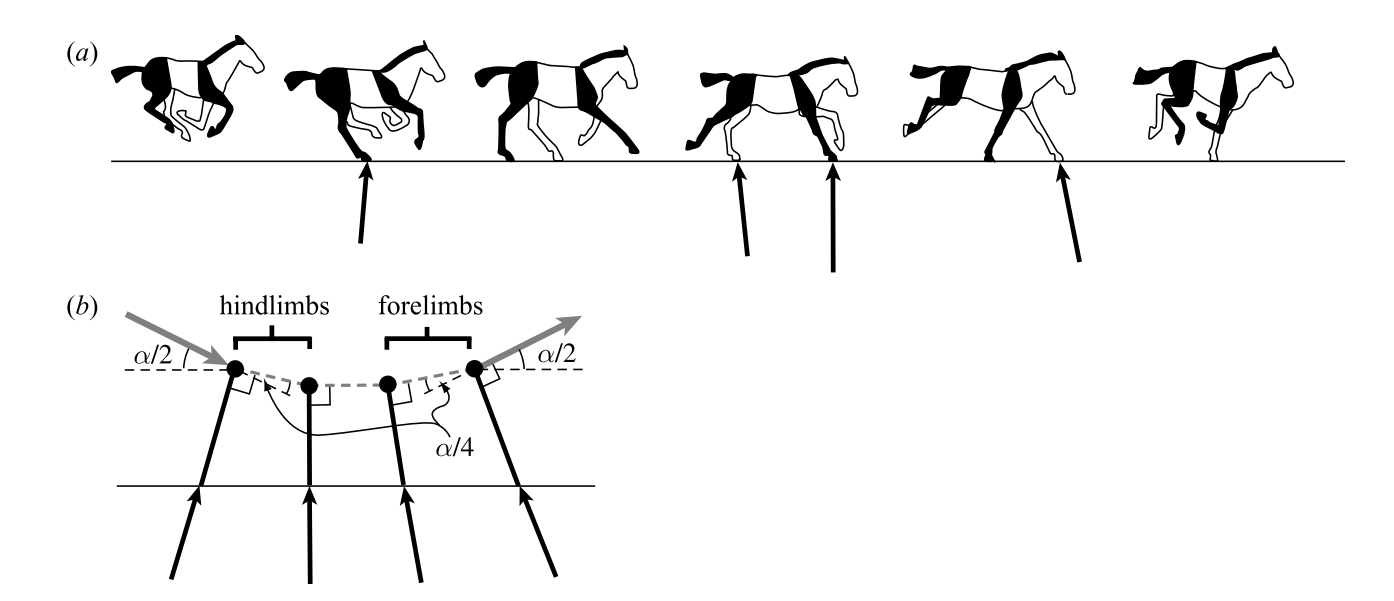
\includegraphics[width=140mm]{figs/HorseGallop}
  \caption{Horse transverse gallop}
  \label{horse}
\end{figure}

\begin{figure}[h]
  \centering
  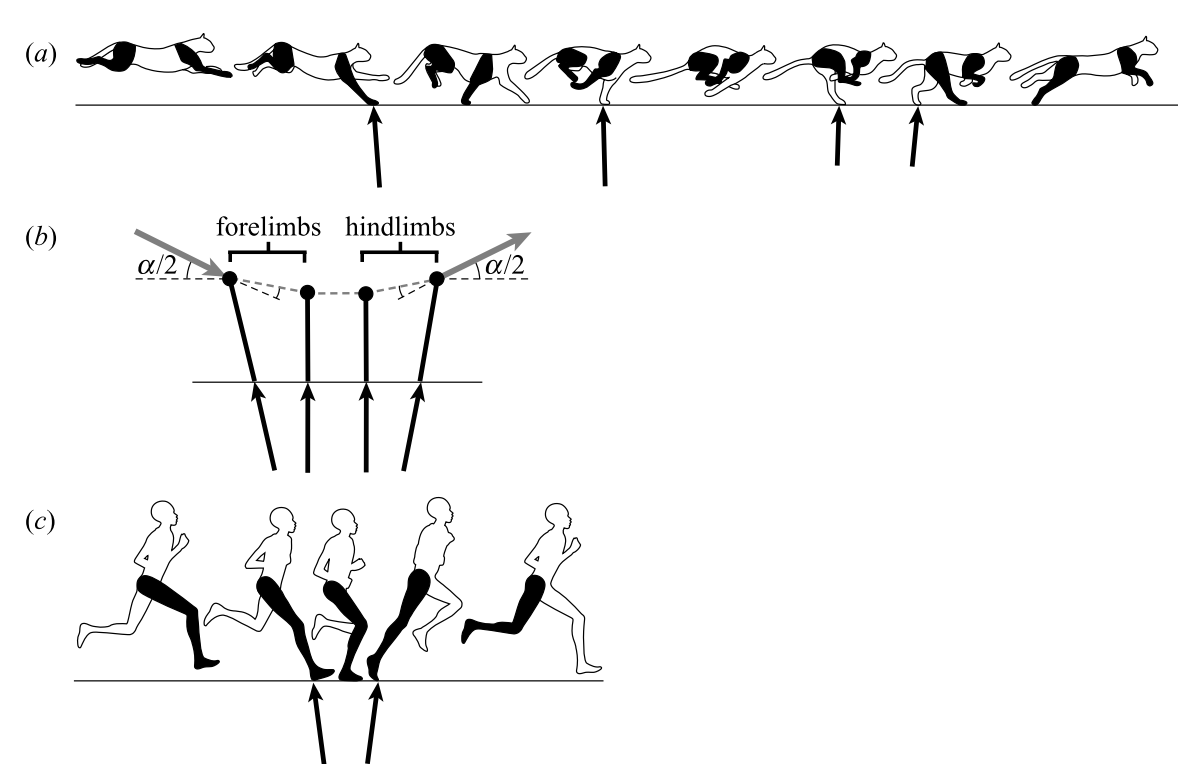
\includegraphics[width=140mm]{figs/CheetahGallop}
  \caption{Cheetah rotary gallop}
  \label{cheetah}
\end{figure}

\subsection*{Summary}
\begin{itemize}
\item The sequence of four-beat gallop (either rotary or transverse) helps the animal distribute over four impacts the direction change of an angle $\alpha$. Each contact contributes with a direction change of $\alpha/4$, regardless which leg is actually performing each impact.

\item The all purpose of a galloping gait is to \textbf{redirect the trajectory of the CoM} from forward-downward (at the end of the aerial phase) to an upward-forward (at the end of the cycle) direction. Rather than the \textit{rotary or transverse gallop} one should pay more attention to which limb initiate first the CoM trajectory transition. As a matter of fact when the forelimbs initiate this change of direction the resulting gait is a cheetah-like rotary (or lateral) gallop while when the hind legs initiate this result in a transverse (or diagonal) gallop. \textbf{The lateral coordination is of smaller importance} since both gaits can be realized even with perfectly parallel hind and front legs (\textbf{half-bound} if only the hind legs are coordinated and \textbf{bound} if also the front limbs are coordinated).

\item We can see in figure \ref{horse} (b) and \ref{cheetah} (b) that both transverse and rotary gallop achieve the same redirection of the CoM trajectory dury the cycle but the leg sequence and the direction of the ground reaction forces are completely different. \textbf{The GRF of the rotary gallop is more similar to the GRFs observed on human gaits}. Therefore the gallop \textbf{achieves in four impacts the same spring like behavior obtained by humans in one single stance.}

\item In order achieve the same kinetic energy at the  start and at the end of the cycle there are two methods: (a) storing the energy and give it back at the end of the stance (spring-like model); (b) reducing the energy loss in the first place (\textbf{pseudo-elastic model}). The latter model is based on the observation that: \textbf{a single limb that changes length in a manner that minimizes impulse along its axis could have much the same effect as a large number of limbs, each of a different length, acting in a sequence}.\\
The gallop works as a combination of spring-like and pseudo-elastic model.

\end{itemize}